\subsection{Comparação entre os codificadores}
\label{sec:codificadores}

No teste, os \num{11} codificadores ficam entre \num{25.95} e \qty{28.83}{\cm} de erro 3-D médio, faixa de \qty{2.89}{\cm}, com MAE médio de \num{12.63} a \qty{14.14}{\cm} e RMSE combinado de \num{18.55} a \qty{20.64}{\cm} (Tabela~\ref{tab:codificadores}). Os quatro primeiros, GATv2-cascata (\qty{25.95}{\cm}), GPS-cascata (\qty{26.06}{\cm}), GATv2 (\qty{26.08}{\cm}) e GPS (\qty{26.27}{\cm}), diferem em até \qty{0.32}{\cm}.

\begin{table}[H]
  \centering
  \caption{Os \num{11} codificadores da comparação final, com capacidade equiparada a \num{1843395} parâmetros, em ordem crescente de erro 3-D médio nos \num{937} eventos de teste; MAE médio, RMSE combinado e erro 3-D médio em cm. $D$: largura dos estados dos nós; $B$: lote escolhido pela sonda de memória (\num{128}, \num{256} ou \num{512} linhas de treino espelhadas, que correspondem, respectivamente, a \num{22250}, \num{11150} e \num{5600} passos de otimização em \num{50} épocas), com as taxas de aprendizado multiplicadas por $B$/\num{128}. $^{\dagger}$: não lê os atributos das arestas. Os quatro primeiros não se distinguem pela reamostragem pareada (Figura~\ref{fig:diferenca_pareada}).}
  \label{tab:codificadores}
  \begin{tabular}{@{}l S[table-format=3.0] S[table-format=1.3] S[table-format=3.0] S[table-format=2.2] S[table-format=2.2] S[table-format=2.2]@{}}
\toprule
 & {} & {Parâmetros} & {} & {MAE} & {RMSE} & {Erro 3-D} \\
Codificador & {$D$} & {(\num{e6})} & {$B$} & {médio (cm)} & {comb.\ (cm)} & {médio (cm)} \\
\midrule
GATv2-cascata & 212 & 1.869 & 128 & 12.63 & 18.64 & 25.95 \\
GPS-cascata & 132 & 1.874 & 128 & 12.79 & 18.69 & 26.06 \\
GATv2 & 204 & 1.819 & 128 & 12.74 & 18.80 & 26.08 \\
GPS & 128 & 1.843 & 256 & 12.95 & 18.55 & 26.27 \\
GeneralConv & 280 & 1.833 & 256 & 12.86 & 18.94 & 26.43 \\
ResGatedGCN$^{\dagger}$ & 292 & 1.841 & 512 & 13.07 & 19.02 & 26.71 \\
GraphSAGE$^{\dagger}$ & 400 & 1.840 & 512 & 13.23 & 19.01 & 26.92 \\
EdgeConv$^{\dagger}$ & 685 & 1.843 & 128 & 13.46 & 20.23 & 27.67 \\
PNA & 147 & 1.841 & 512 & 13.52 & 19.57 & 27.68 \\
GINE & 395 & 1.844 & 512 & 13.81 & 20.21 & 28.23 \\
GINE-cascata & 404 & 1.843 & 512 & 14.14 & 20.64 & 28.83 \\
\bottomrule
\end{tabular}

\end{table}

As diferenças pareadas do erro 3-D médio em relação ao GATv2-cascata são de \qty[retain-explicit-plus]{+0.12}{\cm} (\num{-0.30} a \qty{0.54}{\cm}) para o GPS-cascata, \qty[retain-explicit-plus]{+0.13}{\cm} (\num{-0.28} a \qty{0.55}{\cm}) para o GATv2 e \qty[retain-explicit-plus]{+0.32}{\cm} (\num{-0.12} a \qty{0.77}{\cm}) para o GPS, intervalos que contêm o zero; do GeneralConv em diante (\qty[retain-explicit-plus]{+0.48}{\cm}; \num{0.02} a \qty{0.95}{\cm}), os intervalos ficam acima de zero, sem correção para comparações múltiplas (Figura~\ref{fig:diferenca_pareada}). O GATv2-cascata tem o menor erro 3-D médio em \qty{56.9}{\percent} das reamostras; o GPS, com o menor RMSE combinado (\qty{18.55}{\cm}), lidera essa métrica em \qty{61.8}{\percent} delas; o menor erro de validação é do GATv2 (\qty{25.72}{\cm}). Não há, portanto, um melhor codificador estabelecido. A seguir, o GATv2-cascata representa o grupo dos quatro melhores; foi escolhido pela métrica de teste, o que favorece seu erro de teste, e treinado uma vez, como os demais.

A parada antecipada (\num{15} épocas sem melhora na validação) não foi acionada; o menor erro de validação ocorreu entre as épocas \num{41} e \num{50}, na última época no GraphSAGE e no GeneralConv. No GATv2-cascata (Figura~\ref{fig:curvas_validacao}), o erro de treino nas linhas espelhadas termina em \qty{21.91}{\cm}, e os erros de validação e de teste concordam (\num{25.96} e \qty{25.95}{\cm}).

\begin{figure}[H]
  \centering
  \begin{subfigure}[t]{0.485\textwidth}
    \centering
    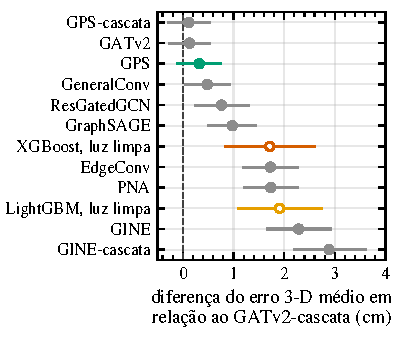
\includegraphics{figures/diferenca_pareada.pdf}
    \caption{Diferença do erro 3-D médio de teste em relação ao do GATv2-cascata, com intervalo de \qty{95}{\percent} por reamostragem \textit{boot\-strap} pareada (\num{10000} reamostras dos \num{937} eventos de teste); o GPS, de menor RMSE combinado, em verde; \mbox{XGBoost} e \mbox{LightGBM} na luz limpa, com marcador vazado. Diferenças positivas indicam erro maior que o do GATv2-cascata; os intervalos do GPS-cascata, do GATv2 e do GPS contêm o zero.}
    \label{fig:diferenca_pareada}
  \end{subfigure}\hfill
  \begin{subfigure}[t]{0.485\textwidth}
    \centering
    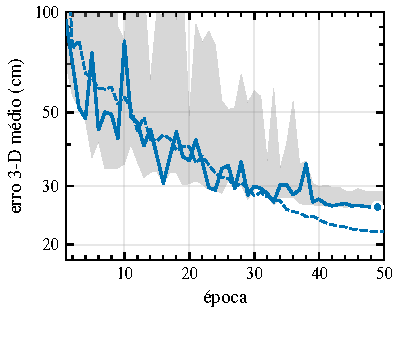
\includegraphics{figures/curvas_validacao.pdf}
    \caption{Erro 3-D médio por época, em escala logarítmica: faixa sombreada entre o menor e o maior erro de validação dos \num{11} codificadores e, para o GATv2-cascata, as curvas de validação (contínua) e de treino nas linhas espelhadas (tracejada), com marcador na época de menor erro de validação. Ficam acima da escala o valor de treino da primeira época e o limite superior da faixa em várias épocas da primeira metade do treino.}
    \label{fig:curvas_validacao}
  \end{subfigure}
  \caption{Comparação entre os \num{11} codificadores com capacidade equiparada: (a) diferenças nos \num{937} eventos de teste; (b) curvas de treinamento.}
  \label{fig:par_codificadores}
\end{figure}

Os três codificadores que não leem os atributos das arestas ficam no meio da Tabela~\ref{tab:codificadores}: ResGatedGCN em sexto, GraphSAGE em sétimo e EdgeConv em oitavo. Os cinco treinados com lote \num{512} (\num{5600} passos) ocupam as posições 6, 7, 9, 10 e 11, e os três primeiros usaram lote \num{128} (\num{22250} passos): a comparação iguala o número de parâmetros, mas não separa o efeito do operador do efeito do orçamento de otimização.
